\documentclass[journal]{IEEEtran}

\usepackage{cite}
\usepackage{amsmath,amssymb,amsfonts}
\usepackage{algorithmic}

\usepackage{graphicx}
\graphicspath{{../../Dissertacao/figuras/}}

\usepackage{textcomp}
\usepackage{xcolor}
\usepackage{booktabs}                        % AAB inserido
\usepackage[utf8]{inputenc}                  % AAB inserido
\usepackage{rotating}                        % AAB inserido

\usepackage{bbm}
\usepackage[binary-units]{siunitx}

\usepackage[caption=false,font=footnotesize]{subfig}
\DeclareMathOperator{\traco}{tr}



\begin{document}
\title{Fusion of Evidences in Intensities Channels for Edge Detection in PolSAR Images}
\author{Anderson A.\ de Borba, Maurício Marengoni, and Alejandro C.\ Frery,~\IEEEmembership{Senior Member,~IEEE}%
\thanks{A.\ A.\ de Borba is with the Dept.\ Engenharia Elétrica e Computação, Universidade Presbiteriana Mackenzie (UPM), and with IBMEC-SP, São Paulo, Brazil. anderson.borba@ibmec.edu.br}
\thanks{M.\ Marengoni is with the Dept.\ Engenharia Elétrica e Computação,
UPM, São Paulo, Brazil. mauricio.marengoni@mackenzie.br}
\thanks{A.\ C.\ Frery is with the Laboratório de Computação Científica e Análise Numérica (LaCCAN), Universidade Federal de Alagoas (UFAL), Maceió, Brazil. acfrery@laccan.ufal.br}}

\maketitle

\begin{abstract}
Synthetic Polarimetric Aperture Radar (PolSAR) sensors have reached an essential position in the area of remote sensing. 
The images coming from PolSAR sensors are contaminated with speckle noise, making their processing and analysis challenging tasks. 
The present study discusses a detection method based on the fusion of evidence obtained in the intensity (hh), (hv), and (vv) channels of PolSAR multi look images. 
The method consists of detecting transition points in the thinnest range of data that covers two regions using the maximum likelihood with estimates of the parameters from the Wishart distribution. 
The fusion methods used are the simple mean, the discrete wavelet (DWT), and stationary (SWT) transform, the principal component analysis (PCA), the ROC statistic, and a multi-resolution method based on singular values (SVD). 
The results indicate an assessment of the influence of each intensity channel in the merging of evidence with possible paths for future research.
\end{abstract}

\begin{IEEEkeywords}
PolSAR, edge detection, maximum likelihood estimation, fusion
\end{IEEEkeywords}

\section{Introduction}\label{sec_01}

\IEEEPARstart{W}{e present}
results on the detection and fusion of edge evidence applied to Polarimetric Synthetic Aperture Radar (PolSAR) images.

Among the available edge detection techniques for PolSAR images, it is worth mentioning:
a) Gradient-based techniques can be found in Refs.~\cite{tlb, obw, flmc, fyf}. They present difficulties due to speckle. For this reason, the treatment of speckle-noise is crucial, giving rise to methods that work by filtering this type of noise Refs.~\cite{ lee, law, cgaf}; 
b) Methods using Markov chains, Ref.~\cite{bf} have intensive use of computational processing;
c) The use of deep learning can be observed in the following Refs.~\cite{bac, ztmxzxf, tabmm, sglmla}, and;
d) techniques based on statistical modeling have been used in border detection, Refs.~\cite{gmbf, fbgm, horrit}.

The article follows the statistical modeling approach using the techniques described in Refs.~\cite{fbgm, nhfc, bmf_2019} to find the edge evidence. As well as, o process the fusing of this information is described in Refs.~\cite{mit, sg}.

This work aims to show the feasibility of a procedure to edge detection in the PolSAR image. The intention is to understand and quantify the importance of the information provided by each channel to improve the edge detection process.

The article is structured as follows.
Section~\ref{sec_02} describes statistical modeling and edge detection for PolSAR data.
Section~\ref{sec_03} describes the approach to edge evidence fusing.
Section~\ref{sec_04} presents the numerical results.
Finally, Section~\ref{sec_05} concludes the work with observations, future directions of research, and the feasibility of detecting edges in each channel of a PolSAR images.

\section{Statistical modeling for PolSAR data}\label{sec_02}

%Fully polarimetric SAR systems transmit orthogonally polarized microwave pulses and measure orthogonal components of the received signal. For each pixel, there is a matrix of scattering, such that the entries are complex numbers. The matrix describes the transformation from the transmitted electromagnetic field to the received electromagnetic field and can be represented as
%\begin{equation*}
% \left[
%\begin{array}{c}
%	E_{\text{h}}^{\text{r}}   \\
%	E_{\text{v}}^{\text{r}}    
%\end{array}
%\right]
% = \frac{e^{\hat{\imath} kr}}{r}\left[
%\begin{array}{cc}
%	S_\text{hh}   & S_\text{hv}   \\
%	S_\text{vh}   & S_\text{vv}   
%\end{array}
%\right]
% \left[
%\begin{array}{c}
%	E_{\text{h}}^{\text{t}}   \\
%	E_{\text{v}}^{\text{t}}    
%\end{array}
%\right],
%\end{equation*}
%where $k$ denotes the wave number, $\hat{\imath}$ is unit imaginary number, and $r$ is the distance between the radar and the target. 
%
%The electromagnetic field with components $E_{\text{i}}^{\text{j}}$ has a subscribed index denoting horizontal (h) or vertical (v) polarization, while the superscript index indicates the received (r) or transmitted (t) wave. Defining $S_\text{ij}$ as the complex scattering coefficients, such that the indices $\text{i}$ and $\text{j}$ are associated with the reception and transmission of waves, for example, the scattering coefficient $S_\text{hv}$ is associated with the wave transmitted in the vertical direction (v) and received in the horizontal direction (h).
%
%The complex scattering matrix $\mathbf{S}$ is defined by
%\begin{equation}
%\mathbf{S} = \left[
%\begin{array}{cc}
%	S_\text{hh}   & S_\text{hv}   \\
%	S_\text{vh}   & S_\text{vv}   
%\end{array}
%\right],
%\label{eq_01}
%\end{equation}
%and if the medium of propagation of waves is reciprocal, then the reciprocity theorem, Ref.~\cite{lp}, allows to state the scattering matrix as being Hermitian.  In this way, the scattering matrix~(\ref{eq_01}) can be represented by the vector $\mathbf{s}=[S_\text{hh},S_\text{hv},S_{\text{vv}}]^T$.
%
%Following Refs.~\cite{good, lee}, the distribution of $\mathbf{s}$ is assumed to be  Gaussian circular complex multivariate with zero mean, and probability density function (pdf) given by:
%\begin{equation}
%    f_{\mathbf{s}}(\mathbf{s};\mathbf{\Sigma})=\frac{1}{\pi^3|\mathbf{\Sigma}|} \exp(-\mathbf{s}^\text{H}\mathbf{\Sigma}^{-1}\mathbf{s}),
%    \label{eq_02}
%\end{equation}
%where $|\cdot|$ is the determinant, 
%the superscript index $\text{H}$ denotes the conjugate complex number, 
%and $\mathbf{\Sigma}$ is the covariance matrix of $\mathbf{s}$ such that $\mathbf{\Sigma}=E[\mathbf{ss}^\text{H}]$, where $E[\cdot]$ denotes the expected value. 
% 
%The statistical modeling described so far deals only with single-look modeling. However, polarimetric images are usually subjected to multi-look processing in order to improve the signal-to-noise ratio. 
%For this purpose, Refs.~\cite{good, ade} show that estimated positive definite Hermitian matrices are obtained by computing the average of $L$ independent samples of the same scene, resulting in the estimated sample covariance matrix:
%\begin{equation}
%    \mathbf{Z}=\frac{1}{L}\sum_{\ell=1}^{L} {\mathbf{s}_\ell}{\mathbf{s}_\ell}^\text{H},
%    \label{eq_03}
%\end{equation}
%where $\mathbf{s}_\ell$, $\ell = 1, \dots, L$, are $L$ independent samples of complex vectors distributed as $\mathbf{s}$.
%
%This statistical modeling has been confirmed for a variety of the polarimetric SAR data, and it contains all the necessary information to characterize the backscatter according to Refs.~\cite{sarabendi,mfp}
%\subsection{Multilook Wishart density function}

Multi-looked fully polarimetric data follow the Wishart distribution with probability density function defined by:
\begin{equation}
    f_{\mathbf{Z}}(\mathbf{Z};\mathbf{\Sigma},L)=\frac{L^{mL}|\mathbf{Z}|^{L-m}}{|\mathbf{\Sigma_{s}}|^{L}\Gamma_m(L)} \exp(-L\traco(\mathbf{\Sigma}^{-1}\mathbf{Z})),
    \label{eq_04}
\end{equation} 
where, $\traco(\cdot)$ is the trace operator of a matrix, $\Gamma_m(L)$ is a multivariate Gamma function defined by
\begin{equation*}
	\Gamma_m(L)=\pi^{\frac{1}{2}m(m-1)} \prod_{i=0}^{m-1}\Gamma(L-i),
\end{equation*}
and $\Gamma(\cdot)$ is the Gamma function.
In this study, $m=3$ is considered. 
This situation is denoted by $\mathbf{Z}\sim W(\mathbf{\Sigma}, L)$, which satisfies $E[\mathbf{Z}]=\mathbf{\Sigma}$. 
This assumption usually holds on targets where the speckle is fully developed.

\subsection{Edge Detection}

Most of the usual techniques for edge detection, e.g., 
Sobel, Canny, Laplacian of Gaussian (LoG) and pyramidal LoG, assume additive Gaussian noise and, thus, they are ineffective for PolSAR imagery.The noise in these kinds of images is multiplicative, making edge detection in SAR images a challenging task.

The main idea for edge detection is based on Ref.~\cite{nhfc, gmbf} and show how to detect the transition point in a thin strip between two regions of the image. The transition point is considered as edge evidence. 

The following procedure is proposed:
\begin{enumerate}
	\item identify the centroid of a region of interest (ROI) in an automatic, semi-automatic or manual manner;
	\item cast rays from the centroid to the outside of the area;
	\item collect data around the rays using the  Bresenham's midpoint line algorithm, ideally the size of a pixel;
	\item detect points in the data strips which provide evidence of changes in their statistical properties, i.e., a transition point that defines edge evidence;
	\item use the Generalized Simulated Annealing (GenSA) method, Ref.~\cite{xgsh}, to find maximum points in the functions of interest;
	\item fuse the evidence of detected edges in the (hh), (hv) and (vv) channels.
\end{enumerate}
With this, fully polarized data is not required, only the intensity channels.

\subsection{Maximum Likelihood Estimator (MLE) to Edge Detection}

The method described in this section can be found in the Refs.~\cite{gmbf,nhfc}. For each radial in the region of interest (ROI), a data strip is considered
\begin{equation}\nonumber
	z = (z_1,z_2,\dots,z_N)
\end{equation}
with partition represented by
\begin{equation}\label{func_max_ver_uni_gamma} 
\begin{array}{lll}
	Z_k&\sim& f_Z(z_k;\mu_\text{I},L_\text{I}), k=1,\dots,j\\
	Z_k&\sim& f_Z(z_k;\mu_\text{E},L_\text{E}), k=j+1,\dots,N
\end{array}
\end{equation}
where, for each $k$, $z_k$ is the realization of the random variable $Z_k$, and they are distributed according to their probability density function (PDF). The indices I e E define if the point lies in inside I or external E of region of interest (ROI).

We use the Gamma model to estimate $(\mu_\text{I},L_\text{I})$ and $(\mu_\text{E},L_\text{E})$:
\begin{equation}\label{func_dens_uni_gamma}
	f_Z(z_k;\mu,L)=\frac{L^{L}z_k^{L-1}}{\mu^{L}\Gamma(L)} \exp\Big\{-L\frac{z_k}{\mu}\Big\}.
\end{equation}
Applying the natural logarithm on both sides of~\eqref{func_dens_uni_gamma}, and performing  the necessary algebra,  the function is found
\begin{equation}\label{func_max_ver_uni_gamma}
\begin{split}
	\ln f_Z(z_k;\mu,L)&= L\ln L +(L - 1) \ln z_k-L \ln \mu \\
	 	                  &{}- \ln \Gamma(L) -\frac{L}{\mu} z_k.\\
\end{split}
\end{equation}

The objective of the method is to find the transition point in each radial data strip .
For this, we consider the function of maximum likelihood $\ell$ for each partition of the data:
\begin{equation}\nonumber
\ell(j;\mu, L)=\sum_{k=1}^{j}\ln f_{Z}(z_k;\mu,L)
             +\sum_{k=j+1}^{N}\ln f_{Z}(Z_k;\mu,L).
\end{equation}
 
Using~\eqref{func_max_ver_uni_gamma} and performing the necessary algebra, the resulting equation is 
\begin{equation}\label{func_l_param}
  \ell(j;\mu, L)=j\ell_1(\mu, L) + (N - j)\ell_2(\mu, L),
 \end{equation}
where
\begin{equation}\label{func_l_param_1_2}
\begin{split}
    \ell_1(\mu, L)&=L\ln L+\frac{L-1}{j}\sum_{k=1}^{j}\ln z_k-L\ln\mu\\
    &{}-\ln\Gamma(L) -\frac{L}{j\mu}\sum_{k=1}^{j} z_k,\text{ and}\\
    \ell_2(\mu, L)&=L\ln L+\frac{L-1}{N-j}\sum_{k=j+1}^{N}\ln z_k-L\ln\mu\\
    &{}-\ln\Gamma(L) -\frac{L}{(N-j)\mu}\sum_{k=j+1}^{N} z_k.
 \end{split}
\end{equation}
 
The functions defined in~\eqref{func_l_param_1_2} are used to estimate the parameters by solving the following optimization problems 
\begin{equation}\label{optimiz_l_1}
(\widehat{\mu}_\text{I},\widehat{L}_\text{I})= \arg\max\limits_{(\mu,L)\in \mathrm{R}^{+}\times\mathrm{R}^{+}}\ell_1(\mu,L),
\end{equation}
and
\begin{equation}\label{optimiz_l_2}
(\widehat{\mu}_\text{E},\widehat{L}_\text{E})= \arg\max\limits_{(\mu,L)\in \mathrm{R}^{+}\times\mathrm{R}^{+}}\ell_2(\mu,L).
\end{equation} 

We used the BFGS optimization method~\cite{nw} implemented in the maxLik package~\cite{ht} to estimate $(\widehat{\mu}_I, \widehat{L}_I)$ and $(\widehat{\mu}_E, \widehat{L}_E)$, for every $j$ in the data strip.

At this point, being known the parameters $(\widehat{\mu}_I, \widehat{L}_I)$ and $(\widehat{\mu}_E, \widehat{L}_E)$ is constructed the $\ell$ function based on~\eqref{func_l_param} as follows,
\begin{equation}\label{l_com_paremetros}
 \begin{split}
\ell&(j;\widehat{\mu}_I, \widehat{L}_I,\widehat{\mu}_E, \widehat{L}_E)=j\Bigg[  \widehat{L}_I(\ln \widehat{L}_I -\ln \widehat{\mu}_I) \\
                                          &{}- \ln \Gamma(\widehat{L}_I) + \frac{\widehat{L}_I  - 1}{j} \sum_{k=1}^{j}  \ln z_k -\frac{\widehat{L}_I}{j\widehat{\mu}_I} \sum_{k=1}^{j}   z_k\Bigg] \\
                                   &{}+(N-j)\Bigg[\widehat{L}_E(\ln \widehat{L}_E - \ln \widehat{\mu}_E)\\
                                   &{}-\ln \Gamma(\widehat{L}_E) + \frac{\widehat{L}_E - 1}{N-j} \sum_{k=j+1}^{N}\ln z_k
                                   -\frac{\widehat{L}_E}{(N-j)\widehat{\mu}_E} \sum_{k=j+1}^{N}z_k\Bigg]. \\
 \end{split}
 \end{equation}
 
We used a Generalized Simulated Annealing method (GenSA~\cite{xgsh}) to find  
$$
\widehat{\jmath}= \arg\max\limits_{j\in [\min_s,N-\min_s]}\ell(j;\widehat{\mu}_I, \widehat{L}_I,\widehat{\mu}_E, \widehat{L}_E),
$$ 
in which $\min_s$ is a minimum sample size that we set to $14$.

In this section, it was shown how to estimate a transition point in the data range. This transition point is defined as edge evidence. 

\section{Methods of fusion of edge evidence}\label{sec_03}

In this section, the methods of fusion of edge evidence used in numerical tests are described. The simple average, stationary wavelet transform (SWT), principal components analysis PCA, and ROC statistics fusion methods are summarized on Ref.\cite{bmf_2019}. However, more details are found in the references Ref.~\cite{n_r,mit,gs} and,~\cite{fawcett}. The discrete wavelet transform and singular value decomposition (SVD) methods are described in the sequence.

\subsection{Multi-Resolution Discrete Wavelet Transform DWT Fusion} 
This section is based on Ref.~\cite{n_r}. In general form, DWT filter is applied separately in vertical and horizontal directions and down-sampled by a factor of two in the image I. In this way, the image is filtered by the low pass filter L in the vertical direction and the high pass filter H in the horizontal direction and then down-sampled by a factor of two to create the coefficients matrices $\text{I}_\text{L}$ and $\text{I}_\text{H}$. After this, the decomposition $\text{I}_\text{L}$ and $\text{I}_\text{H}$ are again submitted to the low pass and high pass filters in the both direction and newly down-sampled by a factor of two to create sub-images named $\text{I}_\text{LL}$,$\text{I}_\text{LH}$, $\text{I}_\text{HL}$ and $\text{I}_\text{HH}$. The successive levels of decomposition can be achieved by repeating this procedure.

The DWT fusion method can be described by the following steps:
\begin{enumerate}
\item Calculate the DWT decomposition by getting $\text{I}_\text{HH}$, $\text{I}_\text{HL}$, $\text{I}_\text{LH}$ and $\text{I}_\text{LL}$ for each channel;
\item in the decomposition, $\text{I}_\text{HH}$ the arithmetic mean of all channels is realized, pixel by pixel, and in the decomposition $\text{I}_\text{HL}$, $\text{I}_\text{LH}$, and $\text{I}_\text{LL}$, the maximum is found between of all channel, pixel by pixel, finding a new operators $\bar{\text{I}}_\text{HH}$, $\bar{\text{I}}_\text{HL}$, $\bar{\text{I}}_\text{LH}$, and $\bar{\text{I}}_\text{LL}$;
\item the image with the fusing of the edge evidence $\text{IF}(x,y)$ is performing the reverse DWT transformation.  
\end{enumerate}

\subsection{Multi-Resolution Singular Value Decomposition SVD Fusion - MSVD}
This section is based on Ref.~\cite{naidu}. Multi-Resolution Singular Value Decomposition SVD Fusion works of similar manner them DWT method.  The difference in the two methods consists in to change the DWT filters to the SVD filters. The SVD fusion method can be summarized to the following steps:
\begin{enumerate}
\item Organize the data in a matrices $X_\ell$ with dimension $4\times\text{MN}$ according to the reference Ref.~\cite{naidu}. The dimension MN is the row number multiply to the  column number of the image PolSAR, and $\ell$ is the level of resolution to set;  
\item find the SVD decomposition to matrix $T=X_\ell X_\ell^T=U_\ell S^2 U_\ell^T$, where $s(1)\geq s(2) \geq s(3) \geq s(4)$ compose the singular value matrix $S$;
\item put $\widehat{X}_\ell=U_\ell^TX_\ell$ and transform the lines this matrix in new matrices with dimensions $\frac{\text{M}}{2}\times\frac{\text{N}}{2}$, named respectively $\{\Phi_\ell, \Psi_\ell^\text{V}, \Psi_\ell^\text{H}, \Psi_\ell^\text{D}\}$. In the next level of decomposition, the $\widehat{X}_\ell$ is replaced by $\Phi_\ell$ until to reach the level L. The MSVD method may be represented as:
\begin{equation}\label{msvd_iter}
\widehat{X}\leftarrow \left\{\Phi_L,\{\Psi_\ell^\text{V},\Psi_\ell^\text{H},\Psi_\ell^\text{D} \}_{\ell=1}^L,\{U_\ell\}_{\ell=1}^L \right\}
\end{equation}
\item After to apply the MSVD to level $\ell$ previously defined is realized the fusion process in the following manner. In the operators $\Phi_\ell^\text{V}$, $\Phi_\ell^\text{H}$ and $\Phi_\ell^\text{D}$, the maximum is found between of all channel, pixel to pixel, resulting in new operators $\bar{\Phi}_\ell^\text{V}$, $\bar{\Phi}_\ell^\text{H}$ and $\bar{\Phi}_\ell^\text{D}$. The other operators $\Psi_\ell$, and $U_\ell$, are averaged to all the channels. There is a  flowchart to  explain the process on Ref.~\cite{naidu};
\item the image with the fusing of the edge evidence $\text{IF}(x,y)$ is performing to the SVD transformation resulting in the above process. 
\end{enumerate}
\section{Numerical results}\label{sec_04}

\subsection{Real PolSAR image}
The PolSAR image of the Flevoland region in the Netherlands is used for the numerical tests. 
Fig.~(\ref{flevoland_radial_4look}) shows the region of interest, with the radial lines for edge detection.

\begin{figure}[hbt]
\centering
	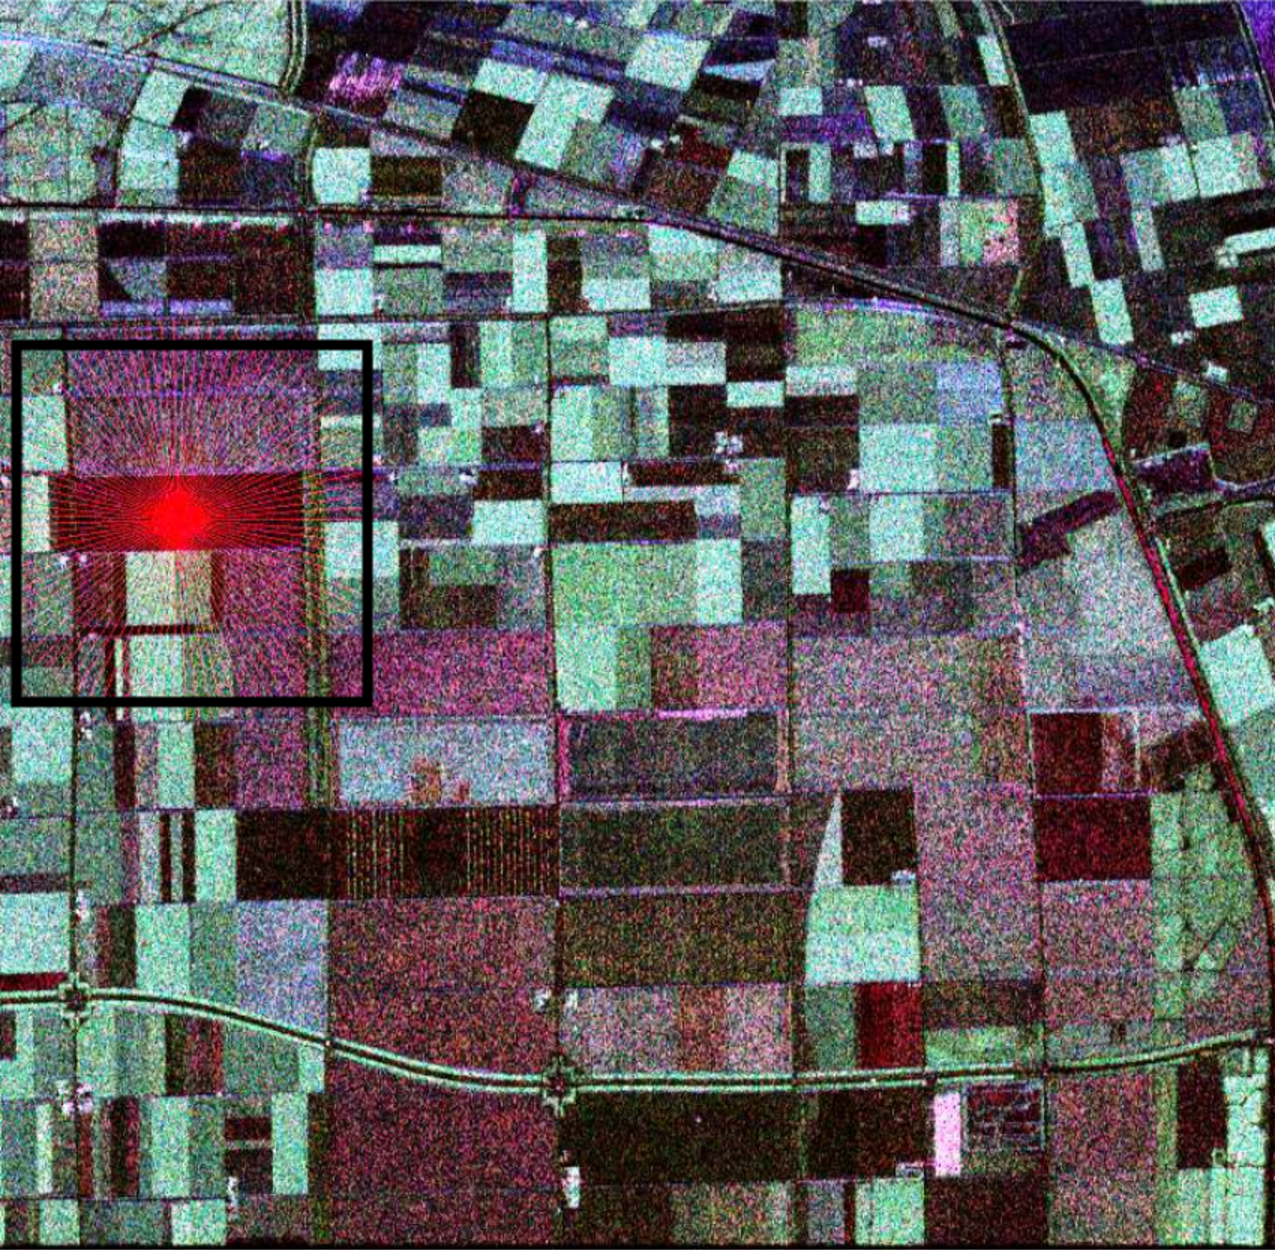
\includegraphics[width=\linewidth]{flevoland_radial_4_look_black}
	\caption{Region of interest (ROI) in the image of Flevoland.}
\label{flevoland_radial_4look}
\end{figure}

The estimates made in equations~(\ref{optimiz_l_1}) and~(\ref{optimiz_l_2}) and their insertion in equation~(\ref{l_com_paremetros}) generated an oscillation at the ends of each radial, depending on the radial considered. In order to get around the problem, we disregarded some pixels on each side of the chosen radial. In the case of this PolSAR image, after performing some tests, 14 pixels on each side are chosen. Disregarded pixels is possible because the chosen radial has 120 pixels. 

Figs.~\ref{evidencias_hh_hv_vv}\subref{evidencias_hh_hv_vv:a}, \subref{evidencias_hh_hv_vv:b} and~\subref{evidencias_hh_hv_vv:c} show, respectively, the edge evidence in the $\text{hh}$, $\text{hv}$ and $\text{vv}$ channels. For each of these figures, the maximum likelihood estimation (MLE) program is executed.

It is worth noting that GenSA has accurately identified the maximum value of function $\ell(j)$, even in the presence of multiple local maxima. Another important observation concerns the performance of the proposed method in the $\text{hv}$ channel. The method presents a few outliers points, in contrast, the method presents good accuracy in the detection of edges evidence. We can also highlight the best performance when compared to channels $\text{hh}$ and $\text{vv}$. 


   \begin{figure*}[hbt]
	\centering
     \subfloat[Evidences in channel $\text{hh}$ \label{evidencias_hh_hv_vv:a}]{%
       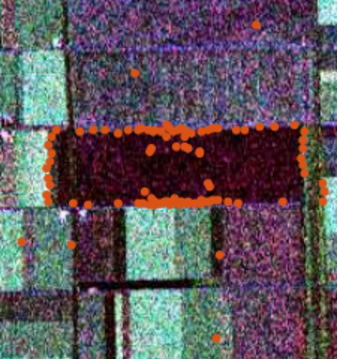
\includegraphics[width=0.32\linewidth]{flevoland_hh_evid_param_L_mu_14_pixel_crop}
     }
     \subfloat[Evidences in channel $\text{hv}$ \label{evidencias_hh_hv_vv:b}]{%
       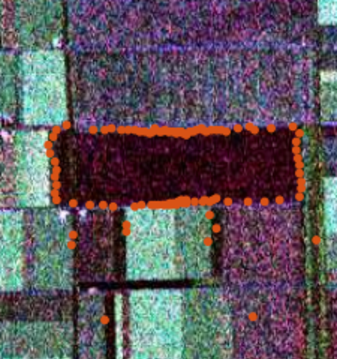
\includegraphics[width=0.32\linewidth]{flevoland_hv_evid_param_L_mu_14_pixel_crop}
     }
     \subfloat[Evidences in channel $\text{vv}$ \label{evidencias_hh_hv_vv:c}]{%
       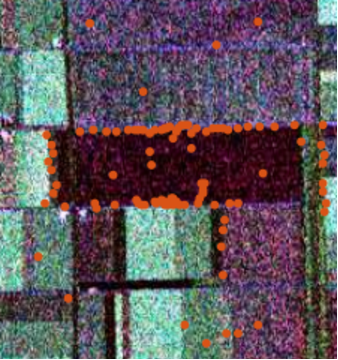
\includegraphics[width=0.32\linewidth]{flevoland_vv_evid_param_L_mu_14_pixel_crop}
     }
     \caption{Edges evidences 14 pixel range}
     \label{evidencias_hh_hv_vv} 
   \end{figure*}

Figs.~\ref{fusion_met}\subref{fusion_met:a}, \subref{fusion_met:b}, \subref{fusion_met:c}, and~\subref{fusion_met:d} show, respectively, the results of fusing these evidences. 

The simple average and PCA methods have similar performances to indicate pixels as edges. The time to perform the methods is shown in the table~(\ref{metrica_de_tempo}). Thus, we can see that the time for the PCA method is 2.19 times longer than the simple average.  

The MSVD method shows excellent performance to indicate pixels of edges; the number of pixels outliers is much smaller than the other methods. The significant disadvantage of the MSVD method is the runtime. We can see in the table~(\ref{metrica_de_tempo}) that it has the highest time.

The ROC Fusion showed edge pixels with good accuracy and a small number of outliers but no show pixels that are edges. One way to get around this problem would be to increase the number of channels considered, as well as use other probability density functions (PDF).

The post-processing is an option to be used in all the fusion methods. An idea can be found in Ref.~\cite{gmbf}. 



\begin{figure*}[hbt]
	\centering
     \subfloat[Average fusion\label{fusion_met:a}]{%
       %\includegraphics[width=0.2\textwidth]{example-image-a}
       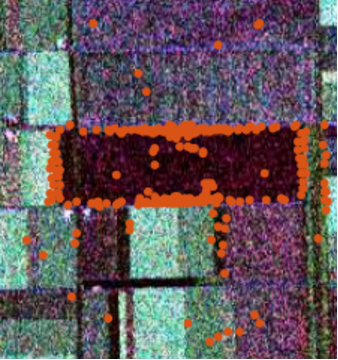
\includegraphics[width=0.32\linewidth]{flevoland_fus_media_param_L_mu_14_pixel_crop}
     }
     \subfloat[SWT fusion\label{fusion_met:b}]{%
       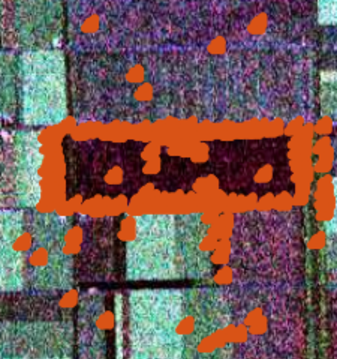
\includegraphics[width=0.32\linewidth]{flevoland_fus_swt_param_L_mu_14_pixel_crop}
     }
     \subfloat[PCA fusion \label{fusion_met:c}]{%
       %\includegraphics[width=0.2\textwidth]{example-image-a}
       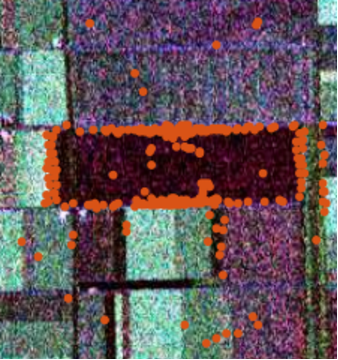
\includegraphics[width=0.32\linewidth]{flevoland_fus_pca_param_L_mu_14_pixel_crop}       
     }\\
     \subfloat[ROC fusion\label{fusion_met:d}]{%
       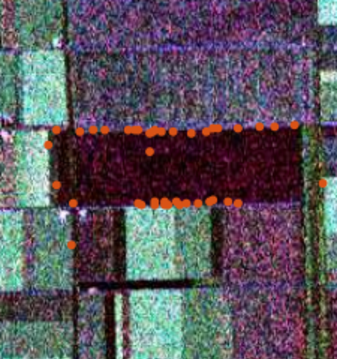
\includegraphics[width=0.32\linewidth]{flevoland_fus_roc_param_L_mu_14_pixel_crop}
     }
     \subfloat[DWT fusion\label{fusion_met:e}]{%
       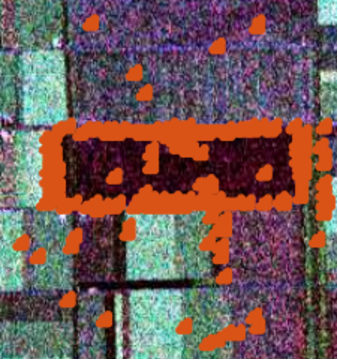
\includegraphics[width=0.32\linewidth]{flevoland_fus_dwt_param_L_mu_14_pixel_crop}
     }
     \subfloat[MSVD fusion\label{fusion_met:f}]{%
       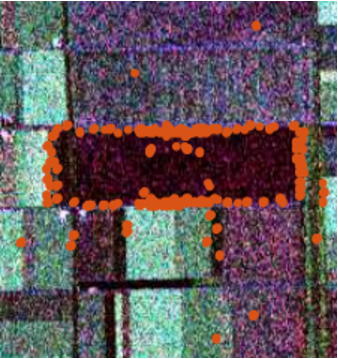
\includegraphics[width=0.32\linewidth]{flevoland_fus_svd_param_L_mu_14_pixel_crop}
     }
     \caption{Fusion methods}
     \label{fusion_met}
\end{figure*}

\subsection{Implementation Details}

We run our programs on a Intel\copyright\ Core i7-9750HQ CPU \SI{2.6}{\giga\hertz} \SI{16}{\giga\byte} RAM computer.  
The method for detecting edge evidence defined with maximum likelihood estimation (MLE) is programmed in R language; on the other hand, the fusion methods are programmed in Matlab language. 
Table~\ref{metrica_de_tempo} shows the computational cost of each of the fusion methods.

\subsection{Processing times} 

This section is constructed a table of the processing time to fusion's methods. The measurement of time was performed only for the fusion method, disregarding the time for the method that finds the evidence of edges, because it is the same for all fusion's methods. The measurement was performed by running the fusion method 20 times and performing the average of these times. The result is shown in the first row of the table (\ref{metrica_de_tempo}), the second row of the table  (\ref{metrica_de_tempo}) was constructed by choosing the shortest time of the methods as the reference time (TR). The other times shown in the table are related to the reference time (TR).   


\begin{table}[hbt]
	\centering
	\tiny
	\caption{Processing times.}\label{metrica_de_tempo}
\begin{tabular}{@{}lllllll@{}} \toprule
	Method       & Average    &   PCA      &  ROC      & DWT       &  SWT        &  MSVD \\ \midrule
	Time (s)      & 0.00858185 & 0.01880955 &0.39989020 &0.07938820 &  0.18071635 & 1.11195710  \\
    Ref. time     & TR & 2.19TR &46.59TR & 9.25TR   & 21.05TR & 129.57TR  \\ \bottomrule
\end{tabular}
\end{table}


\section{Conclusion}\label{sec_05}

Initially, evidence of edges was found using the maximum likelihood method and BFGS to estimate the $L$ and $\mu$ parameters. Later we used this parameter in the maximum likelihood method; at this point, the GenSA method for estimation of edge evidence is applied. In the article, three intensity channels are used to apply the maximum likelihood methods showing excellent accuracy on the actual image of a Flevoland region. We can conclude that the maximum likelihood method in the (hv) channel has superior performance compared to (hh) and (vv) channels.

It is essential to point out that the maximum likelihood method when inserting the $L$ and $\mu$ parameters results in a non-smooth function presenting many local maxima. The difficulty of using the classical optimization methods in this kind function is known, then to get around this problem is applied the simulated annealing method because it is appropriate to optimize non-differentiate functions.

The fusion methods like simple average, SWT, PCA, ROC, DWT, and MSVD are applied to the results of the maximum likelihood methods on each channel. The purpose of applying the fusion methods is to obtain better edge detection accuracy and measure the importance of each channel in the final fusion result.  In this last sense, we can notice that mainly the (vv) channel does not contribute to obtaining a good accuracy of the fusion methods.

Finally, three observations are highlighted; the ROC statistic can be improved by increasing the number of probability density functions for the intensity channels, the weight adjustment for the channels or the choice of the best channels for the fusion of edge evidence, and the use of post-processing on the images coming from the fusion. All these ideas are work in progress.

\bibliographystyle{IEEEtran}
\bibliography{../../../Text/bibliografia}
\end{document}
